\documentclass[9pt,twocolumn,twoside,lineno]{pnas-new}
% Use the lineno option to display guide line numbers if required.

\templatetype{pnasresearcharticle} % Choose template 
% {pnasresearcharticle} = Template for a two-column research article
% {pnasmathematics} %= Template for a one-column mathematics article
% {pnasinvited} %= Template for a PNAS invited submission

\title{Reintroduction of resistant frogs facilitates landscape-scale recovery in the presence of a lethal fungal disease}

% Use letters for affiliations, numbers to show equal authorship (if applicable) and to indicate the corresponding author
\author[a,b]{Roland A. Knapp}
\author[c,1]{Mark Q. Wilber} 
\author[d,e,1]{Allison Q. Byrne}
\author[f,g]{Maxwell B. Joseph}
\author[a,b]{Thomas C. Smith}
\author[d,e,h]{Andrew P. Rothstein}
\author[i]{Robert L. Grasso}
\author[d,e]{Erica Bree Rosenblum}

\affil[a]{Sierra Nevada Aquatic Research Laboratory, University of California, Mammoth Lakes, CA, 93546}
\affil[b]{Earth Research Institute, University of California, Santa Barbara, CA, 93106-3060}
\affil[c]{School of Natural Resources, University of Tennessee Institute of Agriculture, Knoxville, TN, 37996}
\affil[d]{Department of Environmental Science, Policy, and Management, University of California - Berkeley, Berkeley, CA, 94720-3114}
\affil[e]{Museum of Vertebrate Zoology, University of California - Berkeley, Berkeley, CA, 94720-3160}
\affil[f]{Earth Lab, University of Colorado, Boulder, CO, 80303}
\affil[g]{Current affiliation: Planet, San Francisco, CA, 94107}
\affil[h]{Current affiliation: Ginkgo Bioworks, Boston, MA, 02210}
\affil[i]{Resources Management and Science, Yosemite National Park, El Portal, CA, 95318}

% Please give the surname of the lead author for the running footer
\leadauthor{Knapp} 

% Please add a significance statement to explain the relevance of your work
\significancestatement{Understanding how species persist despite accelerating global change is
critical for the conservation of biodiversity. Emerging infectious
diseases can have particularly devastating impacts, and few options
typically exist to reverse these effects. We used large-scale
reintroductions of disease-resistant individuals in an effort to recover
a once-common frog species driven to the brink of extinction by a
disease that has recently devastated global amphibian biodiversity.
Introduction of resistant frogs allowed reestablishment of populations
in the presence of disease. In addition, resistance appears to have a
genetic basis and is consistent with evolution following exposure of
frogs to Bd. The evolution of resistance and reintroductions of
resistant individuals could play an important role in biodiversity
conservation in our rapidly changing world.}

% Please include corresponding author, author contribution and author declaration information
\authorcontributions{}
\authordeclaration{}
\equalauthors{\textsuperscript{1}M.W. contributed equally to this work with A.B.}
\correspondingauthor{\textsuperscript{2}To whom correspondence should be addressed. E-mail: roland.knapp@ucsb.edu}

% At least three keywords are required at submission. Please provide three to five keywords, separated by the pipe symbol.
\keywords{} 

\begin{abstract}
Vast alteration of the biosphere by humans is causing a sixth mass
extinction, driven in part by an increase in emerging infectious
diseases. The emergence of the lethal fungal pathogen
(\emph{Batrachochytrium dendrobatidis}; ``Bd'') has devastated global
amphibian biodiversity, with hundreds of species experiencing declines
or extinctions. Given that there are no broadly applicable methods to
reverse these impacts in the wild, the future of many amphibians appears
grim. The once-common mountain yellow-legged (MYL) frog is emblematic of
amphibians threatened by Bd. Although most MYL frog populations are
extirpated following disease outbreaks, some persist and eventually
recover. Frogs in these recovering populations have increased resistance
against Bd infection, consistent with evolution of resistant genotypes
and/or acquired immunity. We conducted a 15-year landscape-scale
reintroduction study and show that frogs collected from recovering
populations and reintroduced to vacant habitats can reestablish
populations despite the presence of Bd. In addition, results from
viability modeling suggest that many reintroduced populations have a low
probability of extinction over 50 years. To better understand the role
of evolution in frog resistance, we compared the genomes of MYL frogs
from Bd-naive and recovering populations. We found substantial
differences between these categories, including changes in immune
function loci that may confer increased resistance, consistent with
evolutionary changes in response to Bd exposure. These results provide a
rare example of how reintroduction of resistant individuals can allow
the landscape-scale recovery of disease-impacted species. This example
has broad implications for the many taxa worldwide that are threatened
with extinction by novel pathogens.
\end{abstract}

\dates{This manuscript was compiled on \today}
% \doi{\url{www.pnas.org/cgi/doi/10.1073/pnas.XXXXXXXXXX}}

\begin{document}

\maketitle
\thispagestyle{firststyle}
\ifthenelse{\boolean{shortarticle}}{\ifthenelse{\boolean{singlecolumn}}{\abscontentformatted}{\abscontent}}{}

\dropcap{H}uman activities are increasingly impacting global biodiversity (1),
with important implications for ecosystem resilience and human welfare
(2). One consequence of human alteration of the biosphere is an increase
in emerging infectious diseases (3, 4). Such diseases pose a severe
threat to wildlife populations (5), and have caused dramatic declines
and extinctions in a wide range of taxa, including echinoderms, mammals,
birds, and amphibians (6--9). Amphibians are experiencing particularly
devastating impacts of disease due to the recent emergence and global
spread of the highly virulent amphibian chytrid fungus,
\emph{Batrachochytrium dendrobatidis} (Bd) (8, 10). By one estimate,
hundreds of species have experienced Bd-caused declines, and numerous
susceptible taxa are extinct in the wild (8). These impacts to global
biodiversity may be unprecedented, and highlight the importance of
understanding mechanisms of species persistence in the presence of
emerging diseases (11).

Evidence of natural recovery in the many Bd-impacted amphibian
populations is surprisingly rare (for notable exceptions, see 12, 13,
14), suggesting that disease-caused declines will be difficult to
reverse. This apparent low resilience to disease effects may be due to
the limited ability of many amphibians to develop Bd resistance and/or
tolerance, which in turn, could also lessen the effectiveness of
potential Bd mitigation strategies. Following pathogen arrival in a host
population, resistance (ability to limit pathogen burden) and tolerance
(ability to limit the harm caused by a particular burden) are key
mechanisms to reduce disease impacts (15) and facilitate population
persistence and recovery (16). Host immunity and evolution both play
important roles in the development of resistance and tolerance, and
utilizing these factors would seem a promising approach to developing
effective strategies to mitigate disease impacts in the wild (17, 18).
However, several aspects of the amphibian-Bd system present difficult
obstacles, including (i) the general inability of amphibians to mount an
effective immune response against Bd infection (19--21), and (ii) the
apparent rarity of evolution of more resistant/tolerant genotypes (but
see 22, 23). These factors suggest that reintroduction of amphibians
into sites to reestablish populations extirpated by Bd will often result
not in population recovery, but instead in the rapid reinfection and
mortality of the introduced animals and/or their progeny (24--27). If
true, the future of many amphibian species threatened by Bd appears
bleak.

The mountain yellow-legged (MYL) frog, composed of the sister species
\emph{Rana muscosa} and \emph{Rana sierrae} (28), is emblematic of the
global declines of amphibians caused by Bd (8). Once the most common
amphibian in the high elevation portion of California's Sierra Nevada
mountains (USA, 29), during the past century this frog has disappeared
from more than 90\% of its historical range (28). Due to the severity of
its decline and the increasing probability of extinction, both species
are now listed as ``endangered'' under the U.S. Endangered Species Act.
In the Sierra Nevada, this decline was initiated by the introduction of
non-native trout into the extensive historically-fishless region (30,
31) starting in the late 1800s. The arrival of Bd in the mid-1900s and
its subsequent spread (32) caused additional large-scale population
extirpations (33, 34). These Bd-caused declines are fundamentally
different from the fish-caused declines because fish eradication is
feasible (35) and results in the rapid recovery of frog populations (36,
37). In contrast, Bd appears to persist in habitats even in the absence
of amphibian hosts (38), and therefore represents a long-term alteration
of invaded ecosystems that amphibians will need to overcome to
reestablish populations.

Despite the catastrophic impact of Bd on MYL frogs, wherein most
Bd-naive populations are extirpated following Bd arrival (33), some
populations have persisted after epizootics (during which Bd infection
intensity on frogs is very high, 39) and are now recovering
(Figure~\ref{fig-recovery-model}) (14). Frogs in these recovering
populations show reduced susceptibility to Bd infection (14), with
infection intensity (``load'') on adults consistently in the
low-to-moderate range (39--41). This reduced susceptibility is evident
even under controlled laboratory conditions (14), indicative of host
resistance against Bd infection (and not simply an effect of factors
external to individual frogs, e.g., environmental conditions). In
addition to frogs from recovering populations having higher resistance
to Bd infection than those from naive populations, they could also have
higher tolerance, but no data are currently available to evaluate this
possibility. Therefore, we focus on resistance throughout this paper.
The observed resistance of MYL frogs could be the result of several
non-mutually exclusive mechanisms, including natural selection for more
resistant genotypes (22, 23), acquired immunity (21), and/or inherent
between-population differences that pre-date Bd exposure. The possible
evolution of MYL frog resistance and subsequent population recovery is
consistent with that expected under ``evolutionary rescue'', whereby
rapid evolutionary change increases the frequency of adaptive alleles
and restores positive population growth (42, 43). This intriguing
possibility also suggests an opportunity to expand recovery beyond the
spatial scale possible under natural recovery by utilizing resistant
frogs from recovering populations in reintroductions to vacant habitats
(Figure~\ref{fig-recovery-model}) (41, 44).

In the current study, we had three primary objectives. First, to
determine whether the reintroduction of resistant MYL frogs obtained
from populations recovering from Bd-caused declines allows the
successful reestablishment of extirpated populations despite ongoing
disease, we conducted a 15-year landscape-scale frog reintroduction
effort (Figure~\ref{fig-recovery-model}). Second, to extend our
inferences of population recovery well beyond the temporal extent of our
reintroduction study, we developed a model to estimate the probability
of persistence for the reintroduced populations over a multi-decadal
period (Figure~\ref{fig-recovery-model}). Third, given the importance of
resistance for frog survival, population establishment, and long-term
viability (this study), we also conducted a genomic study to determine
whether MYL frogs show an evolutionary response to Bd exposure, and
whether these genomic changes are associated with resistance. To
accomplish this objective, we used exome capture methods to identify
genomic regions with consistent differences between frogs from naive
versus recovering populations (Figure~\ref{fig-recovery-model}).

\section*{Results}

\subsection*{Frog population recovery}

To determine whether MYL frogs from recovering populations can be used
to reestablish extirpated populations, we conducted 24 reintroductions
in Yosemite National Park (2006--2020). Each of the reintroductions
involved collection of adult frogs from 1 of 3 recovering, Bd-positive
``donor'' populations and translocating them to 1 of 12 nearby recipient
sites (Figure S1). The donor populations included 2 of
the 5 recovering populations included in the frog evolution study
referenced above (Figure~\ref{fig-allelefrequencies}: population 1 and
4), and these donor populations contributed frogs for 20 of the 24
translocations. Following translocation, we estimated adult survival and
recruitment of new adults from capture-mark-recapture (CMR) surveys and
obtained counts of tadpoles and juveniles from visual encounter surveys
(VES). Across all translocation sites, the duration of survey time
series was 1--16 years (median = 5).

Of the 12 reintroduced populations, 9 (0.75) showed evidence of
successful reproduction in subsequent years, as indicated by the
presence of tadpoles and/or juveniles. For these 9 populations, one or
both life stages were detected in nearly all survey-years following
translocation (proportion of survey-years: median = 0.9, range =
0.29--1). These same populations were also those in which recruitment of
new adults (i.e., progeny of translocated individuals) was detected. As
with early life stages, recruits were detected in the majority of
post-translocation survey-years (proportion of survey-years: median =
0.79, range = 0.12--1). In summary, survey results indicate that
translocations resulted in the establishment of reproducing MYL frog
populations at most recipient sites despite the ongoing presence of Bd.

Bd loads were fairly consistent before versus after translocation, and
loads were nearly always well below the level indicative of severe
chytridiomycosis (i.e., the disease caused by Bd) and associated frog
mortality (Figure S2) (33, 41). Although it
is possible that the observed relatively small changes in load are a
consequence of individuals with high Bd loads dying and therefore being
unavailable for sampling during the post-translocation period, the fact
that there was little difference in pre- versus post-translocation Bd
loads even in those populations that had very high frog survival (70556,
74976; Figure~\ref{fig-translocation-survival},
Figure S2) suggests a true lack of
substantial change in Bd load.

The ultimate measure of reintroduction success is the establishment of a
self-sustaining population. Given that it can take years or even decades
to determine the self-sustainability of a reintroduced population (for
an example in MYL frogs, see 41), the use of proxies is essential for
providing shorter-term insights into reintroduction success and the
factors driving it. Results from our CMR surveys allowed us to
accurately estimate frog survival, including over the entire CMR time
series for each site and during only the 1-year period immediately
following translocation. These estimates were made using site-specific
models analyzed using the mrmr package. We use these estimates to
describe general patterns of frog survival in all translocated cohorts,
and in an among-site meta-analysis of frog survival to identify
important predictors of 1-year frog survival (e.g., Bd load).

Estimates of 1-year frog survival indicate that survival was highly
variable between recipient sites, but relatively constant within
recipient sites (for the subset of sites that received multiple
translocations; Figure~\ref{fig-translocation-survival}). These patterns
indicate an important effect of site characteristics on frog survival.
In addition, 1-year survival was higher for frogs translocated later in
the study period than earlier: 5 of the 7 populations translocated after
2013 had estimated survival \(\ge\) 0.5, compared to only 1 of 5
populations translocated prior to 2013. We suggest this resulted
primarily from our improved ability to choose recipient sites with
higher habitat quality for \emph{R. sierrae} (see \textbf{Materials and
Methods - Frog population recovery - Field methods} for details). This
increased survival has direct implications for population viability (see
\textbf{Results - Long-term population viability}).

The goal of our meta-analysis was to identify important predictors of
1-year frog survival. We were particularly interested in whether Bd load
had a negative effect on adult survival, as would be expected if frogs
were highly susceptible to Bd infection. This analysis was conducted in
a Bayesian framework and included a diversity of site, cohort, and
individual- level characteristics as predictors and 1-year frog survival
(Figure~\ref{fig-translocation-survival}) as the response variable. The
best model of 1-year frog survival identified several important
predictors, but Bd load at the time of translocation was not among them
(Figure S3). Instead, important predictors
included winter severity in the year following translocation (snow\_t1),
site elevation, and donor population (Figure~\ref{fig-cond-effects},
Figure S3). Males had somewhat higher
survival than females, but this effect was small
(Figure~\ref{fig-cond-effects}, Figure S3).
The absence of Bd load as an important predictor of frog survival is
consistent with frogs in recovering populations having sufficient
resistance to suppress Bd loads below harmful levels.

In summary, results from our frog translocation study indicate that
translocations resulted in (i) relatively high 1-year survival of
translocated adults, as well as reproduction and recruitment, at the
majority of recipient sites, (ii) 1-year survival of adults is
influenced by site characteristics, weather conditions, and donor
population (but not Bd load), and (iii) based on the relatively small
changes in Bd load after translocation, loads appear more strongly
influenced by frog characteristics (e.g., resistance) than site
characteristics. Together, these results indicate that frogs
translocated from recovering populations can maintain the benefits of
resistance in non-natal habitats. In addition, in 3 locations where
longer CMR time series allowed us to assess the survival of new adults
recruited to the population, naturally-recruited adults had equivalent
or higher survival probabilities than the originally translocated adults
(Figure S4). This suggests that frog
resistance is maintained across generations. All of the conditions
described above are supportive of population establishment and long-term
population growth.

\subsection*{Long-term population viability}

Results from the frog translocation study indicated that most
populations showed evidence of successful reproduction and recruitment,
and that adult survival was often relatively high (described above).
Although suggestive of population establishment, a decade or more of
surveys may be necessary to confirm that populations are in fact
self-sustaining (41). To extend our inferences of population
establishment beyond those possible from the site-specific CMR data, we
developed a population viability model. Specifically, to test whether
the observed yearly adult survival probabilities in translocated
populations (provided in legend of Figure~\ref{fig-viability}B) were
sufficient for long-term viability, we built a stage-structured matrix
model that captured known frog demography and included demographic and
environmental stochasticity. We parameterized the model using CMR data
from translocated populations and known life history values in this
system (Table S2 SI).

Given observed yearly adult survival probabilities of translocated frogs
(from site-specific mrmr CMR models) and a yearly survival probability
of the year-1 juvenile class (\(\sigma_{J_1}\)) greater than 0.09, at
least six of twelve translocated populations should experience a
long-run growth rate \(\lambda\) greater than 1 in the presence of Bd
(Figure~\ref{fig-viability}A; median predicted \(\lambda\) ranges from
1.19-1.40 for these six populations). These six populations all had
observed yearly adult survival greater than 0.5. As year-1 juvenile
survival probability increased above 0.2, the deterministic long-run
growth rate of eight of twelve population was greater than 1
(Figure~\ref{fig-viability}A).

Even when incorporating (i) demographic stochasticity and (ii)
environmental stochasticity in year-1 juvenile survival and recruitment
(the transition that we expect to be the most subject to environmental
variability in the presence of Bd), populations with high adult survival
are likely to persist over a 50 year time horizon. Our model predicted
that, following a single introduction of 40 adult individuals into a
population, the six populations with the highest adult survival
probabilities (\(\sigma_{A_R} > 0.5\)) had 50-year extinction
probabilities of less than 0.5 when the average year-1 juvenile survival
was greater than 0.10 (Figure~\ref{fig-viability}B). This indicates
strong potential for long-term persistence in the presence of Bd and
environmental variability in survival and recruitment. In contrast, for
the six populations where yearly adult survival probability
\(\sigma_{A_R} < 0.5\), extinction probability over 50 years was always
predicted to be \textgreater{} 50\% regardless of the value of mean
year-1 juvenile survival between 0 and 0.25. To test the validity of our
model predictions, we demonstrated that our stochastic model could
describe the general recovery trajectory of our translocated population
with the longest survey history (Figure~\ref{fig-viability}C;
population 70550, surveyed for 16 years).

In summary, our model demonstrates that given observed yearly adult
survival probabilities of translocated frogs, 50\% of our translocated
populations have a high probability of population growth and long-term
viability in the presence of Bd. This is likely a conservative estimate
because there is evidence that naturally-recruited adults have higher
survival probability than translocated adults
(Figure S4), but we considered these
probabilities to be equal in all but three of our populations where we
had sufficient data to distinguish these different probabilities.

\subsection*{Frog evolution in response to Bd}

Results from the preceding sections indicate the critical role of frog
resistance in post-translocation frog survival, population growth, and
population viability. As such, identifying the mechanisms underlying
this resistance would fill a key gap in our understanding of the factors
that promote population resilience in the presence of disease. Although
natural selection for more resistant frog genotypes, and evolutionary
rescue, may be foundational to the ability of frogs to recover despite
ongoing Bd infection, for MYL frogs the role of disease-mediated
selection in these processes remains unknown.

To determine whether MYL frog populations show genomic patterns
consistent with an evolutionary response to Bd, we compared frog exomes
(i.e., coding region of a genome) between populations with contrasting
histories of Bd exposure. Specifically, we compared frog genomes sampled
in 4 populations that have not yet experienced a Bd-caused epizootic
(``naive'') (45) versus in 5 populations that experienced a Bd epizootic
during the past several decades and have since recovered to varying
degrees (``recovering''; Figure~\ref{fig-allelefrequencies}) (14, 33).
Bd-exposure histories of the 9 study populations are based on 10-20
years of VES and Bd surveillance using skin swabbing (e.g., 14, 45, 46).
Naive populations are characterized by large numbers of adults (i.e,
typically 1000s), Bd prevalence that is generally 0\% except during
occasional Bd failed invasions (during which Bd loads remain very low,
46), and no history of Bd epizootics since we first surveyed these
populations in the late 1990s and early 2000s (45). In contrast,
recovering populations exist in an enzootic state (39), characterized by
smaller numbers of adults (generally \textless{} 100), high Bd
prevalence (often \textgreater{} 80\%, 40), and, in adults, moderate Bd
loads that are typically well below the level expected to cause
mortality (33). Naive and recovering populations can be identified
unambiguously using these differences in Bd prevalence and load.
Finally, there is no potential for frog dispersal between the 9 study
populations due to intervening distances and topography, as well as the
presence of introduced (predatory) fish and fish-induced habitat
fragmentation. (See \textbf{Supporting Information - Frog evolution in
response to Bd - Methods} for additional details regarding the study
design.)

We conducted a principal component analysis (PCA) of the genomic data to
describe the relationships between sampled populations, and then used
two complementary approaches to identify regions of the genome that
differed between naive and recovering populations (i.e., regions under
selection). First, we used a multivariate linear mixed model to evaluate
associations between population type (i.e., naive versus recovering) and
individual variants, including single nucleotide polymorphisms (SNPs)
and insertions/deletions (INDELS), while accounting for population
structure. Second, we used a splined window analysis to identify larger
genomic regions showing differences between population types in
\emph{F\textsubscript{ST}} and nucleotide diversity (\(\pi_{diff}\) =
\(\pi_{naive}\) - \(\pi_{recovering}\)).

Individual frogs clustered into 3 separate groups in principal component
space (Figure S6A SI), and clusters reflected
the species split (i.e., \emph{R. muscosa} versus \emph{R. sierrae}) and
the strong signature of isolation-by-distance that is characteristic of
MYL frogs (47--49). Importantly, each cluster contained at least one
population from both the naive and recovering groups, allowing us to
distinguish allelic associations of individuals sampled in the 2
population types versus allelic associations resulting from population
structure and genetic drift.

Results from the individual variant and splined window analyses show
that recovering populations have signatures of selection on multiple
regions of the genome. The analysis of individual variants identified 11
``outlier'' SNPs (i.e., showing significantly different allele
frequencies between naive versus recovering populations) from 7 distinct
genes across 4 contigs (Figure S6B, C SI; SI
Datasets S1, S2). One of the 7 identified genes (LOC108802036) does not
have an associated annotation. For the outlier SNPs, frequency
differences between the naive and recovering populations ranged from
0.41 to 0.86. Most of these SNPs showed frequency differences in only a
subset of the sampled populations (Figure~\ref{fig-allelefrequencies}A,
B), but the SNP in the RIN3 gene showed consistent differences in
frequencies across all populations (Figure~\ref{fig-allelefrequencies}
C). This is suggestive of parallel selection at this locus across
multiple populations. The other 6 outlier variants showed less
consistent frequency differences across the study populations, but for
these we still found a statistically significant signal of selection in
2 of the 3 genetic clusters (containing populations 5--9;
Figure~\ref{fig-allelefrequencies}, Figure S6A
SI). Therefore, although some outlier variant associations have a more
limited geographic extent than RIN3, they still describe results that
suggest parallel evolutionary changes following Bd exposure.

The splined window analysis identified 33 outlier regions for
\(\pi_{diff}\) and 58 outlier regions for \emph{F\textsubscript{ST}}
(Figure~\ref{fig-spline-manhattan}A, B). Of these, 9 regions were
outliers for both metrics (``shared regions'') and 2 of these shared
regions also contained one or more of the outlier SNPs described above.
A total of 33 annotated genes were found in the 9 shared regions
(Datasets S3, S4). Given this large number of genes, here we focus on
those with the strongest signal of selection and/or immune-related
functions. The largest \(\pi_{diff}\), indicative of directional
selection, occurred in a 163kb region on Contig19, 12.9Mb upstream of
the RIN3 outlier SNP (Figure~\ref{fig-spline-manhattan}C). This region
contains approximately 500 SNPs and one annotated gene called
``interferon-induced very large GTPase 1-like'' (GVINP1). Additionally,
a shared outlier region on Contig1 contained two complement factor genes
(C6 and C7). Interestingly, this region had a large negative
\(\pi_{diff}\) value, consistent with balancing selection. Finally, one
shared outlier region on Contig8 contained one outlier SNP (TCF19) and
was within 360kb of another outlier SNP (VARS)
(Figure~\ref{fig-spline-manhattan}D, Figure S7).
This region (854kb from the beginning of the outlier window to the VARS
SNP) contained a total of 8 annotated genes. In \emph{Xenopus}, five of
these genes occur in the extended major histocompatibility complex (MHC)
Class I region (FLOT1, TUBB, MDC1, CCHCR1, TCF19) and three occur in the
extended MHC Class III region (HSP70, LSM2, VARS) (50). Therefore, this
region under selection is part of the extended MHC Class I and III
complex and shows synteny with other amphibian genomes.

Although the joint processes of Bd-caused population declines and
selection in response to Bd exposure could affect genetic diversity of
recovering populations, we found no consistent differences in
individual-level heterozygosity or population-level \(\pi\) between
naive and recovering populations (see \textbf{Supporting
Information-Frog evolution in response to Bd} for details). Thus,
despite localized selection in particular regions of the genome, we did
not find evidence for reduced genetic diversity across the genome in
recovering populations. In addition, no gene ontology (GO) biological
functions, molecular functions, or cellular processes were
over-represented in either the outlier variants or the 33 genes located
in the overlapping \emph{F\textsubscript{ST}} and \(\pi_{diff}\) splined
windows (see \textbf{Supporting Information-Frog evolution in response
to Bd} for details).

In summary, our genomic results indicate that the exomes of frogs from
naive and recovering study populations show substantial differences,
consistent with parallel evolutionary changes following Bd exposure. The
regions under selection contain several immunologically-relevant genes
and gene families that are directly linked to disease resistance in
other taxa.

\section*{Discussion}

Disease-induced population declines are decimating global biodiversity
(5), but broadly-applicable strategies to recover affected species are
generally lacking (e.g., 17). Here, we tested the possibility that
populations of resistant individuals from naturally recovering
populations can be used to reestablish extirpated populations of the
endangered MYL frog in the presence of a highly virulent fungal pathogen
(Bd). Our results indicate (i) the capacity of reintroduced populations
to become established and eventually recover despite ongoing disease,
(ii) that the recovering populations are likely to persist over a
50-year period, (iii) that there are substantial genomic differences
between naive and recovering MYL frog populations, consistent with
evolutionary change in frogs following Bd exposure, and (iv) that some
of the genomic regions under selection contain genes related to disease
resistance. Collectively, these results
(Figure~\ref{fig-recovery-model}) provide a rare example of amphibian
recovery in the presence of Bd, and have important implications for the
conservation and recovery of amphibians and other taxa worldwide that
are endangered by escalating impacts from emerging infectious diseases.
In light of the generally low success rate of amphibian reintroduction
efforts (51), our success in reestablishing MYL frog populations via
translocation of resistant individuals is striking, and even more so
given that this success occurred despite ongoing infection of frogs with
Bd.

In the following discussion, we follow the sequence of frog recovery
described in Figure~\ref{fig-recovery-model} to structure our key
points. Previous field studies in MYL frogs show that frog-Bd dynamics
and frog survival in the presence of Bd are fundamentally different
between naive and recovering populations. Following the arrival and
establishment of Bd in previously-naive populations, adult frogs develop
high Bd loads that lead to mass die-offs (33). In contrast, in
recovering populations adult frogs typically have low-to-moderate and
relatively constant Bd loads and mass die-offs are not observed (39, 40,
see also Figure S2). The differences in Bd
load of frogs from naive and recovering populations are also observed in
controlled laboratory studies (see Figure 4 in 14), and clearly indicate
that frogs from recovering populations exhibit resistance against Bd
infection. This resistance could in theory be due to several factors,
including natural selection for more resistant genotypes, acquired
immunity, and/or inherent between-population differences that pre-date
Bd exposure, but until now evidence to evaluate the role of evolution
was lacking.

Results from our genomic analyses suggest that natural selection for
adaptive alleles is at least partially responsible for the increased
resistance of frogs in recovering populations. We identified multiple
specific alleles and genomic regions showing signatures of selection
between adjacent naive and recovering MYL frog populations, consistent
with selection following Bd exposure. These analysis are based on
samples collected from virtually all of the MYL frog populations
remaining in a naive state, as well as adjacent recovering populations.
This produced genetic clusters that contained at least one naive and one
recovering population, allowing us to detect selection without the
confounding effects of population structure. Finally, we did not find a
reduction in overall genetic variation in the recovering populations,
suggesting that despite localized selection in the genome, these
populations retain adequate genetic diversity for long-term persistence.

Importantly, some regions that we identified as under selection are
associated with cellular and immunological mechanisms known to
contribute to disease resistance, including in amphibians (52). For
example, the MHC plays an important role in immunity. In our study, we
identified a region that shows evidence of selection in recovering
populations and contains eight genes associated with either the MHC
Class I or Class III regions. These results corroborate numerous
previous studies linking MHC genes to amphibian resistance against Bd
(e.g., 53, 54). Similarly, the region with the strongest indication of
directional selection (as measured by \(\pi_{diff}\)) contains the
interferon-related gene GVINP1. Several previous studies of amphibians
have found this gene to be differentially expressed during Bd infection
(e.g., 23, 55) and in populations differing in Bd susceptibility (23).
This gene is also strongly linked to disease in salmon, explaining a
notable 20\% of the resistance phenotype (56, 57). We also identified a
region, characterized by high \emph{F\textsubscript{ST}} and low
\(\pi_{diff}\), that contained the complement genes C6 and C7. The
complement system plays an important role in innate immunity (58), and
our results could indicate that balancing selection is acting in this
region of the genome to favor a diverse set of alleles, as is known for
C6 in humans (59). Based on the analysis of individual outlier variants,
the RIN3 gene showed a consistent pattern of allele frequency
differences across all nine of the frog populations sampled in this
study, indicating consistent selection in populations distributed across
a wide geographic area. This gene is associated with inflammation
response and in \emph{Xenopus} is highly expressed in wounds (60).
Finally, the outlier variant with the lowest p-value was the
uncharacterized gene LOC108802036. In the genome of another frog
species, this gene is located adjacent to a type I interferon gene
(Np-IFNi2) (61), and together with GVINP1 further suggests the
importance of interferon-related genes in this system. Collectively, the
genes associated with these genomic differences may confer at least some
degree of resistance against Bd infection, an attribute that may be
critically important to population reestablishment and recovery in the
presence of Bd.

Reintroduction of resistant MYL frogs was remarkably successful in
reestablishing viable populations in the presence of Bd. Of the 12
translocated populations, approximately 80\% showed evidence of both
successful reproduction and recruitment of new adults. Year-1 survival
for 12 of the 24 translocated cohorts exceeded 50\%, and \textgreater{}
70\% of translocated cohorts had survival above this 50\% level when the
earliest translocations are excluded (i.e., translocations conducted
when methods were still being refined; see \textbf{Materials and Methods
- Frog population recovery - Field methods} for a brief description of
these refinements). The fact that the relatively low Bd loads and
correspondingly high frog survival was maintained when frogs were moved
from donor populations to recipient sites indicates that these
characteristics of naturally-recovering populations were not solely an
effect of site characteristics, but were also strongly influenced by
resistance inherent in the frogs. Although it could be argued that the
relatively invariant Bd loads before versus after translocation are a
consequence of similar pathogen pressure in the donor and translocated
populations, this is at odds with the fact that in the first year after
translocation frog densities are typically 1-2 orders of magnitude lower
in the translocated versus donor populations and pathogen pressure
should follow a similar pattern. In addition to the maintenance of Bd
load and frog survival between natal and translocation sites, the
relatively high survival of translocated frogs was maintained in their
progeny, as expected if resistance has a genetic basis.

Results from the population viability model were also encouraging. In
particular, translocated populations with \textgreater{} 50\% survival
in the first year post-translocation were predicted to have a low
probability of extinction over 50 years (probability of extinction \(<\)
0.5 when year 1 juvenile survival probability was greater than 0.10).
The viability model highlighted the important role of frog survival in
affecting long-term population viability, and allowed us to extend the
temporal scale of our study beyond the years covered by our
post-translocation surveys. These long-term forecasts are important,
given that reintroduced MYL frog populations may often take decades to
achieve our ultimate goal of self-sustainability (41). Making
well-supported projections about the long-term outcome of reintroduction
efforts from shorter-term information is critically important to the
process of adaptive management of species reintroduction programs (62),
including the one we are carrying out for MYL frogs. Specifically, the
combined results from our reintroduction study and viability modeling
indicate that survival of frogs in the first year following
translocation is an effective proxy of longer-term survival and
population viability. In addition, given the repeatability of frog
survival at a site, 1-year frog survival also serves as an effective
proxy of site quality (i.e., the ability of a site to support high frog
survival and a viable frog population over the long term). This proxy of
site quality is important in the MYL frog system because accurately
predicting the ability of a site to support a viable frog population
\emph{a priori} remains difficult, even after conducting 24
translocations over 16 years.

Despite the demonstrated resistance of adult MYL frogs against Bd
infection, individual and population-level impacts of Bd are still
evident. In an earlier study of 2 of our 12 translocated populations
(41), Bd infection and load had detectable effects on the survival of
adults and may have influenced population establishment (sites referred
to as ``Alpine'' and ``Subalpine'' in (41) are identified as ``70550''
and ``70505'' in the current study). Applying similar analyses to all 12
of our translocated populations would likely provide a broader
perspective of the ongoing effect of Bd. In addition to these important
but relatively subtle effects of Bd on adults, the impacts on younger
life stages are more apparent. MYL frogs immediately following
metamorphosis (``metamorphs'') are highly susceptible to Bd infection
(63) and as a result experience high mortality (34). This high
susceptibility of metamorphs is documented in numerous species of
anurans, and may result from the poorly developed immune system
characteristic of this life stage (64). In naturally recovering and
translocated MYL frog populations, we suggest that the high mortality of
metamorphs is an important limitation on subsequent recruitment of new
adults. Therefore, although adult MYL frogs appear relatively resistant,
Bd infection continues to have important limiting effects on recovering
populations (see also 65).

The recent emergence of Bd worldwide has contributed to the decline of
hundreds of amphibian species, some of which are now extinct in the wild
(8). This extraordinary impact on global amphibian biodiversity is
compounded by the lack of any effective and broadly applicable
strategies to reverse these impacts (17, 25). Importantly, in addition
to the natural recovery documented for MYL frogs (14), other species are
also showing evidence of post-epizootic recovery in the presence of Bd
(12, 13) and suggest the possibility of also using animals from these
recovering populations to reestablish extirpated populations. As with
MYL frogs, the feasibility and long-term success of such efforts will
depend on the availability of robust donor populations containing
individuals that have the adaptive alleles necessary to allow frog
survival and population growth in the presence of Bd. Despite the
hopeful example of successful reestablishment of MYL frogs despite
ongoing Bd infection, the challenge of recovering hundreds of
Bd-impacted amphibian species globally is a daunting prospect. Although
we now have a proven strategy to reestablish extirpated MYL frog
populations, recovery across their large historical range will require
substantial resources over many decades. The results of this study
provide a hopeful starting point for that endeavor and other future
efforts worldwide.

In our rapidly changing world, evolution is likely to play in important
role in facilitating the resilience of wildlife populations. Whether the
documented disease resistance in MYL frogs and concurrent recovery of
decimated populations provides an airtight example of evolutionary
rescue will likely always be uncertain (given that can never have a
perfect understanding of the past). Regardless, we provide an example
from the wild that suggests that evolution can produce individuals that
harbor adaptive alleles and allow population recovery in a novel (i.e.,
Bd-positive) environment, and show conclusively that individuals from
these recovering populations can be used to reestablish extirpated
populations and expand the scale of natural recovery
(Figure~\ref{fig-recovery-model}). We expect that similar species
recovery actions will be an essential tool in wildlife conservation in
an era of accelerating global change.


\matmethods{
\hypertarget{frog-population-recovery-1}{%
\section*{Frog population recovery}\label{frog-population-recovery-1}}

\hypertarget{field-methods}{%
\subsection*{Field methods}\label{field-methods}}

For the 24 translocations we conducted, we identified donor populations
from which adult frogs (\(\geq\) 40 mm snout-vent length) could be
collected using several years of VES and skin swab collections (14), and
results from population genetic analyses (48). The populations that we
selected contained hundreds to thousands of both \emph{R. sierrae}
adults and tadpoles. These relatively high abundances were the result of
recent increases following previous Bd-caused declines (14). As is
typical for recovering MYL frog populations, Bd prevalence in the donor
populations was high (0.69--0.96) and Bd load (median
log\textsubscript{10}(load) = 3.06--3.78 ITS copies) was two or more
orders of magnitude below the level at which frog mortality is expected
(log\textsubscript{10}(load) \(\approx\) 5.78 copies)(33, 41). Recipient
sites to which frogs were translocated were chosen based on previous
\emph{R. sierrae} presence (determined from VES and/or museum records)
or characteristics that suggested high quality habitat for this species
(66). At the beginning of this study, we had a relatively limited
understanding of the factors that affect habitat quality. In subsequent
years, we improved our site selection process by incorporating new
information about important habitat features, in particular, overwinter
habitats such as submerged boulders and overhanging banks. \emph{R.
sierrae} were absent from all recipient sites prior to the first
translocation.

We conducted 1--4 translocations per site
(Figure~\ref{fig-translocation-survival}, Figure S1)
and each translocated cohort included 18 to 99 frogs (median = 30). In
preparation for each translocation, adult frogs were collected from the
donor population and measured, weighed, swabbed, and PIT tagged. Frogs
were transported to the recipient site either on foot or via helicopter.
Following release, we visited translocated populations approximately
once per month during the summer active season and conducted diurnal CMR
surveys and VES (summer active season is generally July-August but can
start as early as May and end as late as September; range of survey
dates = May-25 to Sep-29, range of translocation dates = Jun-28 to
Sep-02; median number of visits per summer = 2, range = 1--10). CMR
surveys allowed estimation of adult survival, recruitment of new adults,
and adult population size, and VES provided estimates of tadpole and
juvenile abundance. During 2006-2012, we conducted CMR surveys on a
single day (primary period) per site visit, during which we searched all
habitats repeatedly for adult frogs. Frogs were captured using handheld
nets, identified via their PIT tag (or tagged if they were untagged),
measured, weighed, swabbed, and released at the capture location. During
2013-2022, we generally used a robust design in which all habitats were
searched during several consecutive days (median number of secondary
periods per primary period = 3; range = 3--7), and frogs were processed
as described above. However, when the number of frogs detected on the
first survey day was zero or near zero, we typically conducted only a
single-day CMR survey. When using a robust design, within a primary
period, frogs that were captured during more than one secondary period
were measured, weighed, and swabbed during the first capture, and during
subsequent captures were only identified and released.

During each site visit, we conducted VES either immediately before CMR
surveys or during the first day of CMR surveys. VES was conducted by
walking the entire water body perimeter, first 100 m of each inlet and
outlet stream, and any fringing ponds and wetlands, and counting all
\emph{R. sierrae} tadpoles and juveniles. These \emph{R. sierrae} life
stages have high detectability, and counts are highly repeatable and
provide estimates of relative abundance (31).

\hypertarget{frog-counts-and-reproductive-success}{%
\subsection*{Frog counts and reproductive
success}\label{frog-counts-and-reproductive-success}}

For each of the translocated populations, we used the presence of
tadpoles and/or juveniles from VES and counts of new recruits (i.e,
untagged adults) in CMR surveys to provide two measures of successful
reproduction. To calculate the proportion of years in which
tadpoles/juveniles were present at a site, we excluded surveys conducted
in the year of the initial translocation to that site. This exclusion
accounted for the fact that all translocations were conducted after the
breeding period and reproduction would therefore not occur until the
following year. Similarly, to calculate the proportion of years in which
new recruits were present at a site, we excluded surveys conducted
during the 3 years following the initial translocation. This accounted
for the multi-year tadpole and juvenile stages in MYL frogs
(Table S2 SI).

\hypertarget{estimation-of-frog-survival-and-abundance}{%
\subsection*{Estimation of frog survival and
abundance}\label{estimation-of-frog-survival-and-abundance}}

For each translocation site, we estimated survival of translocated
frogs, recruitment of new frogs into the adult population, and adult
population size using a site-specific Bayesian open-population
Jolly-Seber CMR model with known additions to the population (i.e.,
translocated cohorts), as implemented by the mrmr package (67) and using
R Statistical Software (v4.4.4, 68) (see \textbf{Supporting Information
- Frog population recovery - CMR model structure} for details). Briefly,
the model tracks the states of \emph{M} individuals that comprise a
superpopulation made up of real and pseudo-individuals (see 41 for
details). The possible states of individuals include ``not recruited'',
``alive'', and ``dead''. The possible observations of individuals
include ``detected'' and ``not detected''. We assume that individuals
that are in the ``not recruited'' or ``dead'' states are never detected
(i.e., there are no mistakes in the individual PIT tag records). We also
assume that new recruits were the result of within-site reproduction and
not immigration from adjacent populations. This assumption is justified
by the fact that no \emph{R. sierrae} populations were present within
several kilometers of the translocation sites. For all models, we used
mrmr defaults for priors, number of chains (4), and warmup and
post-warmup iterations (2000 for each). We evaluated convergence of the
Markov chain Monte Carlo (MCMC) algorithm using trace plots and
Gelman-Rubin statistics (Rhat).

\hypertarget{predictors-of-post-translocation-frog-survival}{%
\subsection*{Predictors of post-translocation frog
survival}\label{predictors-of-post-translocation-frog-survival}}

To identify important predictors of frog survival following
translocation, we used multilevel Bayesian models (69, 70). Included
predictor variables describe characteristics of sites, translocated
cohorts, and individuals (Bd load, sex, frog size, site elevation,
winter severity in the year of translocation, winter severity in the
year following translocation, donor population, day of year on which a
translocation was conducted, and translocation order). We used 1-year
post-translocation survival estimates from CMR models as the response.
Estimated survival was rounded to integer values to produce a binary
outcome, and modeled with a Bernoulli distribution. Group-level (random)
effects included site\_id, translocation\_id, or translocation\_id
nested within site\_id. We performed all analyses with the rstanarm
package (71) and R Statistical Software (v4.4.4, 68). For all models, we
used default, weakly informative priors, four chains, and 5000
iterations each for warmup and post-warmup. We checked MCMC convergence
using trace plots and Rhat, and evaluated model fit using leave-one-out
cross-validation (72), as implemented by the loo package (73). (See
\textbf{Supporting Information - Frog population recovery - Among-site
survival modeling} for details.)

\hypertarget{changes-in-bd-load-following-translocation}{%
\subsection*{Changes in Bd load following
translocation}\label{changes-in-bd-load-following-translocation}}

We analyzed skin swabs using standard Bd DNA extraction and qPCR methods
(74, see \textbf{Supporting Information-Frog population recovery -
Laboratory methods} for details). To assess the magnitude of changes in
Bd load on frogs following translocation, we compared Bd loads measured
before versus after translocation. Before-translocation loads were
quantified using skin swabs collected from all to-be-translocated frogs
at the donor site on the day before or the day of the translocation.
After-translocation Bd loads were based on all swabs collected from
translocated frogs at the recipient site in the year of and the year
following translocation. Individual frogs and their associated Bd loads
were included in the dataset only if frogs were captured at the
recipient site at least once during the 1-year period following
translocation.

Code to replicate all of the analyses described above is available from
the following GitHub repositories:
\url{https://github.com/SNARL1/translocation};
\url{https://github.com/SNARL1/cmr-analysis}.

\hypertarget{population-viability-modeling}{%
\section*{Population viability
modeling}\label{population-viability-modeling}}

\hypertarget{model-description}{%
\subsection*{Model description}\label{model-description}}

To determine the implications of observed 1-year adult survival on the
long-term viability of populations established via translocation, we
developed a population model for MYL frogs. Our central question was:
How does the magnitude and variation in observed adult survival
probability across translocated populations affect the long-term
persistence probability of populations? We developed a model that
tracked seven state variables of a frog population: density of
translocated adults (\(A_T\)), density of adults naturally recruited
into the population (\(A_R\)), density of first-year tadpoles (\(L_1\)),
density of second-year tadpoles (\(L_2\)), density of third-year
tadpoles (\(L_3\)), density of first-year juveniles (\(J_1\)), and
density of second-year juveniles (\(J_2\)). We divided adults into two
classes \(A_T\) and \(A_R\) because there is evidence that the survival
probability of translocated adults and naturally recruited adults
differs (Figure S4).

We modeled the dynamics of these seven state variables using a
discrete-time, stage-structured model where a time step is one year. The
dynamics are given by equation \ref{eqn:matrix}.

\begin{figure*}\[
\begin{bmatrix}
L_1 \\
L_2 \\
L_3 \\
J_1 \\
J_2 \\
A_R \\ 
A_T
\end{bmatrix}(t + 1) = 
\begin{bmatrix}
  0 & 0 & 0 & 0 & 0 & \sigma_{A_R} p_F F & \sigma_{A_T} p_F F \\
  \sigma_{L1} p_{L1} & 0 & 0 & 0 & 0 & 0 & 0 \\
  0 & \sigma_{L2} p_{L2} & 0 & 0 & 0 & 0 & 0\\
  \sigma_{L1} (1 - p_{L1}) & \sigma_{L2} (1 - p_{L2}) & \sigma_{L3} & 0 & 0 & 0 & 0 \\
  0 & 0 & 0 & \sigma_{J1} p_{J1} & 0 & 0 & 0 \\
  0 & 0 & 0 & \sigma_{J1} (1 - p_{J1}) & \sigma_{J2}  & \sigma_{A_R} & 0 \\
  0 & 0 & 0 & 0 & 0 & 0 & \sigma_{A_T} 
\end{bmatrix} \begin{bmatrix}
L_1 \\
L_2 \\
L_3 \\
J_1 \\
J_2 \\
A_R \\
A_T \\
\end{bmatrix}(t)\numberthis \label{eqn:matrix} 
\]\end{figure*}

The parameters in this model are yearly survival probability
\(\sigma_{\cdot}\) (the subscript ``\(\cdot\)'' indicates a particular
state variable), probability that a female frog reproduces in a given
year \(p_F\), number of eggs produced by a female frog in a year that
successfully hatch \(F\), probability of a first-year tadpole remaining
as a tadpole \(p_{L1}\), probability of a second-year tadpole remaining
as a tadpole \(p_{L2}\), and probability of a first-year juvenile
remaining as a juvenile \(p_{J1}\). First-year juvenile survival and
recruitment \(\sigma_{J1}\) is the parameter that we think is most
influenced by environmental stochasticity.

In this model we ignore density-dependent recruitment because we were
interested in the growth of the population from an initial
reintroduction and whether this growth was sufficient to prevent
extinction over 50 years following the introduction. We also did not
directly consider the dynamics of Bd in this model. We made this
decision because (i) translocated populations are infected with Bd at
high prevalence (41), and (ii) host density does not seem to play a
significant role in multi-year Bd infection dynamics in this system
(46). Thus, ignoring Bd infection dynamics and instead assuming all host
vital rates are in the presence of high Bd prevalence significantly
simplifies the model without much loss of realism. Additional details
are provided in \textbf{Supporting Information - Population viability
modeling}.

\hypertarget{model-analysis}{%
\subsection*{Model analysis}\label{model-analysis}}

After parameterizing our model with CMR-estimated adult frog survival
probabilities and other known vital rates
(Table S2), we performed four analyses. First, we
compute the long-run growth rate \(\lambda\) for each of our 12
translocated populations to determine if the populations were
deterministically predicted to grow or decline in the long-run. Second,
we compute the elasticity of \(\lambda\) to four key model parameters to
quantify how much changes in these parameters affected the long-run
growth rate (Figure S5). This also helped us
determine where in the model environmental variation in juvenile
survival and recruitment would have the largest effects on population
dynamics. Third, we included demographic stochasticity and environmental
stochasticity in \(\sigma_{J_1}\) in our model and simulated the 50-year
viability (i.e., 1 - extinction probability) of populations given an
introduction of 40 adult individuals into an unoccupied habitat.
Finally, we fit our model to our longest translocation trajectory to
confirm that our model could reasonably reproduce the observed recovery
trajectories of MYL frogs following reintroductions. Additional details
are provided in \textbf{Supporting Information - Population viability
modeling}. Code to replicate the analyses can be found at
\url{https://github.com/SNARL1/translocation}.

\hypertarget{frog-evolution-in-response-to-bd-1}{%
\section*{Frog evolution in response to
Bd}\label{frog-evolution-in-response-to-bd-1}}

\hypertarget{sampling-and-sequencing}{%
\subsection*{Sampling and sequencing}\label{sampling-and-sequencing}}

We collected DNA samples via buccal swabbing (75) from 53 \emph{Rana
muscosa}/\emph{Rana sierrae} individuals: 24 from 4 naive populations,
and 29 from 5 recovering populations. These populations are located in
the southern Sierra Nevada, from northern Yosemite National Park to
northern Sequoia National Park (Figure~\ref{fig-allelefrequencies}).
Samples were collected from 5-6 frogs per population. To minimize
potential confounding effects caused by variation in frog genotypes
across latitude (49), we selected sampling sites such that both
population types were represented across similar latitudinal ranges. DNA
was extracted following Qiagen DNEasy manufacturer's protocols. We
sequenced the samples using an exome capture assay as described in (49).
Briefly, genomic libraries were prepared and captured using a custom
Nimblegen capture pool. Capture baits were designed based on the coding
regions of the \emph{R. muscosa} transcriptome (GenBank accession
GKCT00000000). Captured libraries were then pooled and sequenced on a
NovaSeq 6000 150PE Flow Cell S1 at the Vincent J. Coates Genomics
Sequencing Lab at UC Berkeley. Raw sequencing reads are available from
NCBI SRA (PRJNA870451).

\hypertarget{data-pre-processing-and-cleaning}{%
\subsection*{Data pre-processing and
cleaning}\label{data-pre-processing-and-cleaning}}

Raw reads were filtered for adapters and contaminants using fastp (76)
and aligned to the \emph{Rana muscosa} genome (NCBI SRA: SRS6533475
(77)), with repetitive elements masked using bwa (``mem'' mode) (78).
Exact PCR duplicates were marked using Picard. Variants were then called
following GATK best practices (v.4.2.0.0 (79)). Briefly, raw variants
were called for each sample using HaplotypeCaller and combined using
CombineGVCFs. Next, genotypes were jointly called using GenotypeGVCFs.
Variants were then hard filtered using gatk VariantFiltration using the
following parameters to remove low-quality sites: QD \textless{} 2.0, FS
\textgreater{} 40.0, SOR \textgreater{} 3.0, MQ \textless{} 50.0,
MQRankSum \textgreater{} 3.0, MQRankSum \textless{} -3.0, ReadPosRankSum
\textgreater{} 3.0, ReadPosRankSum \textless{} -3.0. This initial filter
resulted in 1,595,206 variant sites across 53 individuals.

We then further filtered our dataset at the individual and variant
level. First, we trimmed our variants to only include those with minor
allele frequency \textgreater{} 0.03, a maximum depth of 250 and minimum
depth of 5, a minimum genotype quality of 20, and a maximum missing
proportion of 0.5. This filter resulted in 427,038 sites, of which
353,172 were SNPs and 73,866 were INDELS. Finally, we trimmed samples
with an average depth across filtered sites \textless{} 7x (n = 3). Our
final dataset included 50 samples, 23 from naive and 27 from recovering
populations, with an average depth of 16.7x (range = 7.4x -- 26.1x).

\hypertarget{data-analysis}{%
\subsection*{Data analysis}\label{data-analysis}}

To visualize the genomic relationships of our populations, we conducted
a PCA using the glPCA function in the adegenet R package (80). To detect
regions of the genome that differed between naive and recovering
populations, i.e., regions under selection, we used two approaches: (1)
a multivariate linear mixed model to evaluate individual variants (SNPs
and INDELs), and (2) a splined window analysis to evaluate larger
genomic regions. For the variant analysis, we first used a stringent
data filter to include only variants with \textless{} 5\% missing data
(missing for no more than 2 individuals), and then calculated the
likelihood ratio statistic for the resulting set of 148,307 high quality
variants across 127 contigs using GEMMA (81). GEMMA calculates and
incorporates a relatedness matrix for input samples, allowing us to
account for relatedness and population structure when calculating
likelihood ratio statistics. We identified variants showing different
allele frequencies between naive versus recovering populations
(``outliers'') using a Bonferroni-corrected significance level of 0.01.
We visualized the results using a Manhattan plot and qqplot. We
developed a more liberal set of outlier variants using a
Bonferroni-corrected significance level of 0.05 and used this set solely
for the gene ontology (GO) analysis (see below and \textbf{Supporting
Information}: Dataset S1, S2).

In the analysis of individual variants, for each outlier variant we
determined whether the variant was synonymous (protein sequence the same
for each variant) or non-synonymous (protein sequence differs between
variants), and where in the gene it was located. To do this, we first
extracted the reference genome sequence surrounding the variant using
the bedtools ``getfasta'' function (82). Next, we re-annotated each
sequence using BLAST to get the predicted gene location based on the
closest annotated reference (83). We then translated each variant to
amino acids and aligned this translation to that of the gene annotation
to ensure proper frame of reference using Geneious (84). After ensuring
proper translation, we characterized variants as within or outside the
coding sequence of the gene and as either synonymous or non-synonymous.

In the splined window analysis, we identified outlier regions using
\emph{F\textsubscript{ST}} and differences in nucleotide diversity
(\(\pi_{diff}\)) between naive and recovering populations. First, we
calculated per-site \emph{F\textsubscript{ST}} between the naive and
recovering individuals for all bi-allelic SNPs in the 30 largest contigs
(98\% of all SNPs) using VCFtools (85). Next, we calculated per-site
nucleotide diversity \(\pi\) separately for individuals from the naive
and recovering populations using VCFtools, then calculated
\(\pi_{diff}\) for each population
(\(\pi_{diff} = \pi_{naive} - \pi_{recovering}\)). We concatenated the
values for \emph{F\textsubscript{ST}} and \(\pi_{diff}\) in order of
size-sorted chromosome number and adjusted the SNP position based on the
relative position in the genome (for more efficient data processing and
to better contextualize the strength of the outlier signals in different
regions of the genome). We then used the GenWin R package (86) to
conduct a splined discrete window analysis for
\emph{F\textsubscript{ST}} and \(\pi_{diff}\). This method calculates
where non-overlapping window boundaries should occur by identifying
inflection points in the spline fitted to \emph{F\textsubscript{ST}} and
\(\pi_{diff}\) values along the genome, therefore balancing false
positive and false negative results that occur using other window-based
methods (86). This method also calculates a W-statistic allowing for
outlier identification. We identified outliers as those with a
W-statistic greater than 4 standard deviations above the mean for
\emph{F\textsubscript{ST}} or above/below the mean for \(\pi_{diff}\).
These standard deviations represent strict criteria to select only the
top \textasciitilde{} 0.3\% of windows. Shared outliers were then
identified as those that were outliers in both analyses, meaning that
they showed (i) high differentiation between naive and recovering
populations, and (ii) differential patterns of nucleotide diversity in
the same region. Finally, we extracted gene transcripts mapped within
each region and retrieved annotation for that region using BLAST
(\textbf{Supporting Information}: Datasets S3, S4).

Code used for genomic analyses and to create figures is available from
the following GitHub repository:
\url{https://github.com/allie128/mylf-selection}.

}


\showmatmethods{} % Display the Materials and Methods section

\acknow{We thank the following for important contributions to this study: E.
Hegeman and A. Lindauer--project and data management, field and
laboratory work; A. Barbella and K. Rose--laboratory work; C. Kamoroff
and numerous summer technicians--field work; staff at Sequoia-Kings
Canyon and Yosemite National Parks, Inyo and Sierra National Forests,
California Department of Fish and Wildlife, U.S. Fish and Wildlife
Service, University of California-Santa Barbara Institutional Animal
Care and Use Committee, and Sierra Nevada Aquatic Research
Laboratory--research permits, logistical support, and/or field
assistance. This project was supported by grants from the National Park
Service (to R.A.K.), Yosemite Conservancy (to R.A.K.), and National
Science Foundation (EF-0723563, to C. Briggs; DEB-1557190, to C. Briggs;
DEB-2133401, to M.Q.W; and DBI-2120084, to C. Richards-Zawacki).}

\showacknow{} % Display the acknowledgments section

% Bibliography
\bibliography{translocation}

\clearpage
\begin{figure*}

{\centering 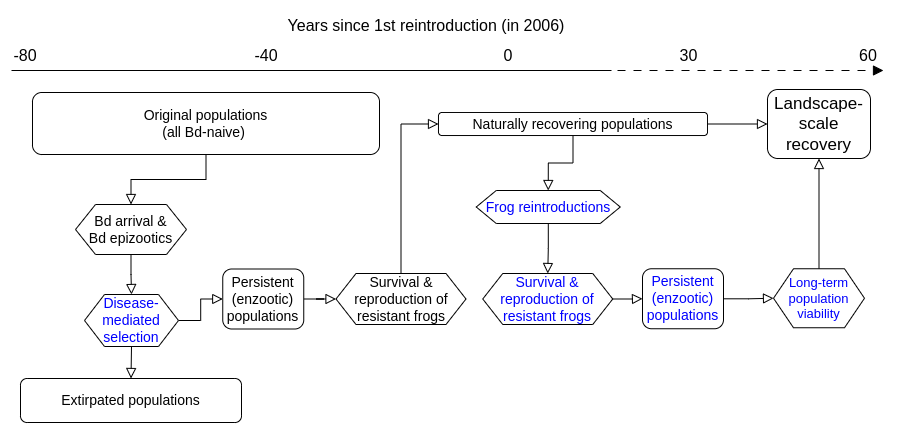
\includegraphics[width=\textwidth]{figures/conceptual_model.png}

}

\caption{\label{fig-recovery-model}For MYL frogs, a conceptual model
depicting the Bd-caused decline and subsequent natural recovery (black
text), facilitated recovery via reintroductions, and the linkages
between these two pathways. Rectangles and hexagons represent outcomes
and processes, respectively. Blue text indicates components that are
included in the current study. The timeline shows the general sequence
of the components, with the dotted portion indicating a projection into
the future.}

\end{figure*}

\newpage

\begin{figure*}

{\centering 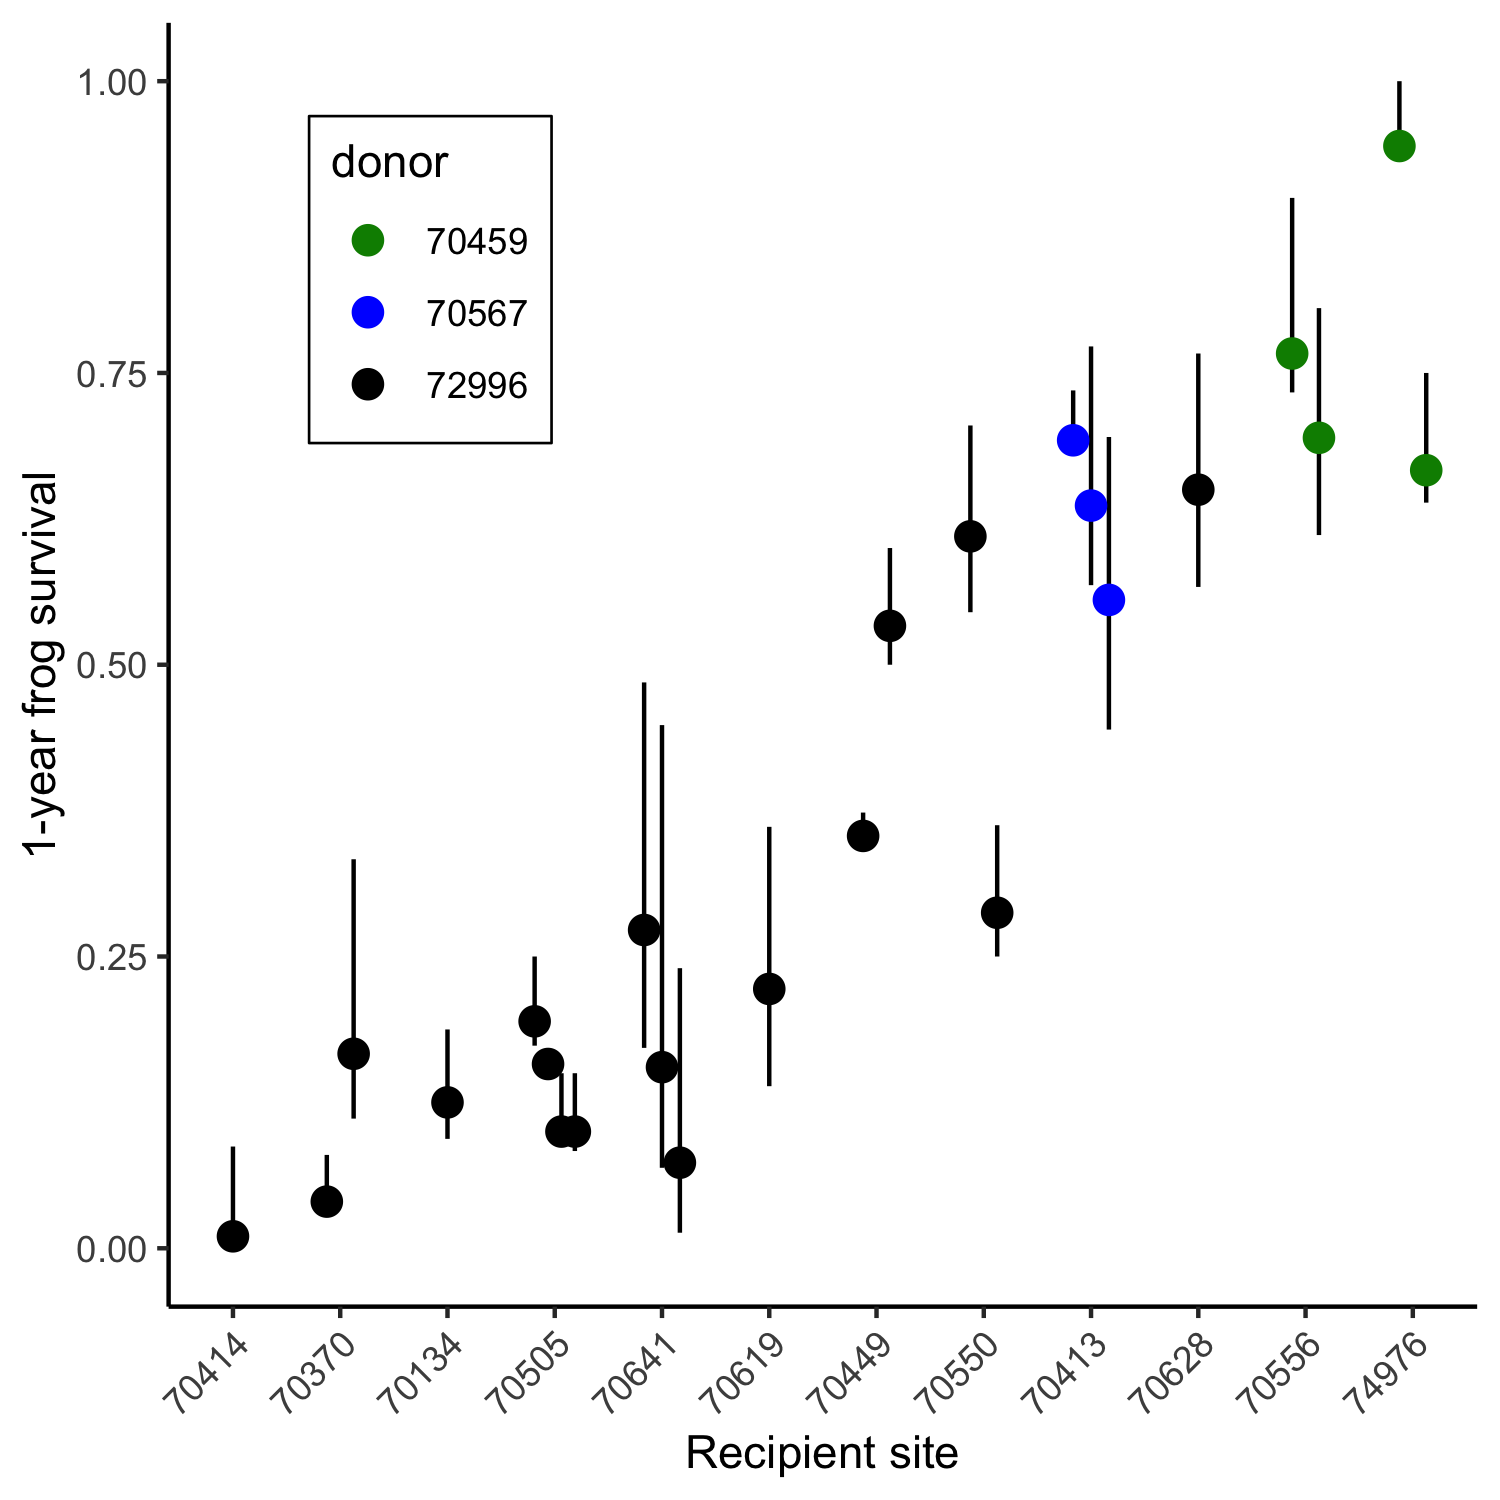
\includegraphics[width=0.5\textwidth]{figures/translocation_survival_bysiteid.png}

}

\caption{\label{fig-translocation-survival}Median 1-year survival for
each cohort of translocated frogs at the 12 recipient sites, as
estimated for each site from the mrmr CMR model. Error bars show the
95\% uncertainty intervals. Sites are arranged along the x-axis using
the average of the median 1-year survival per translocation at each
site. Dot colors indicate the donor population from which frogs in each
translocated cohort were collected. When multiple translocations were
conducted to a site, points and error bars are slightly offset to avoid
overlap.}

\end{figure*}

\newpage

\begin{figure*}

{\centering 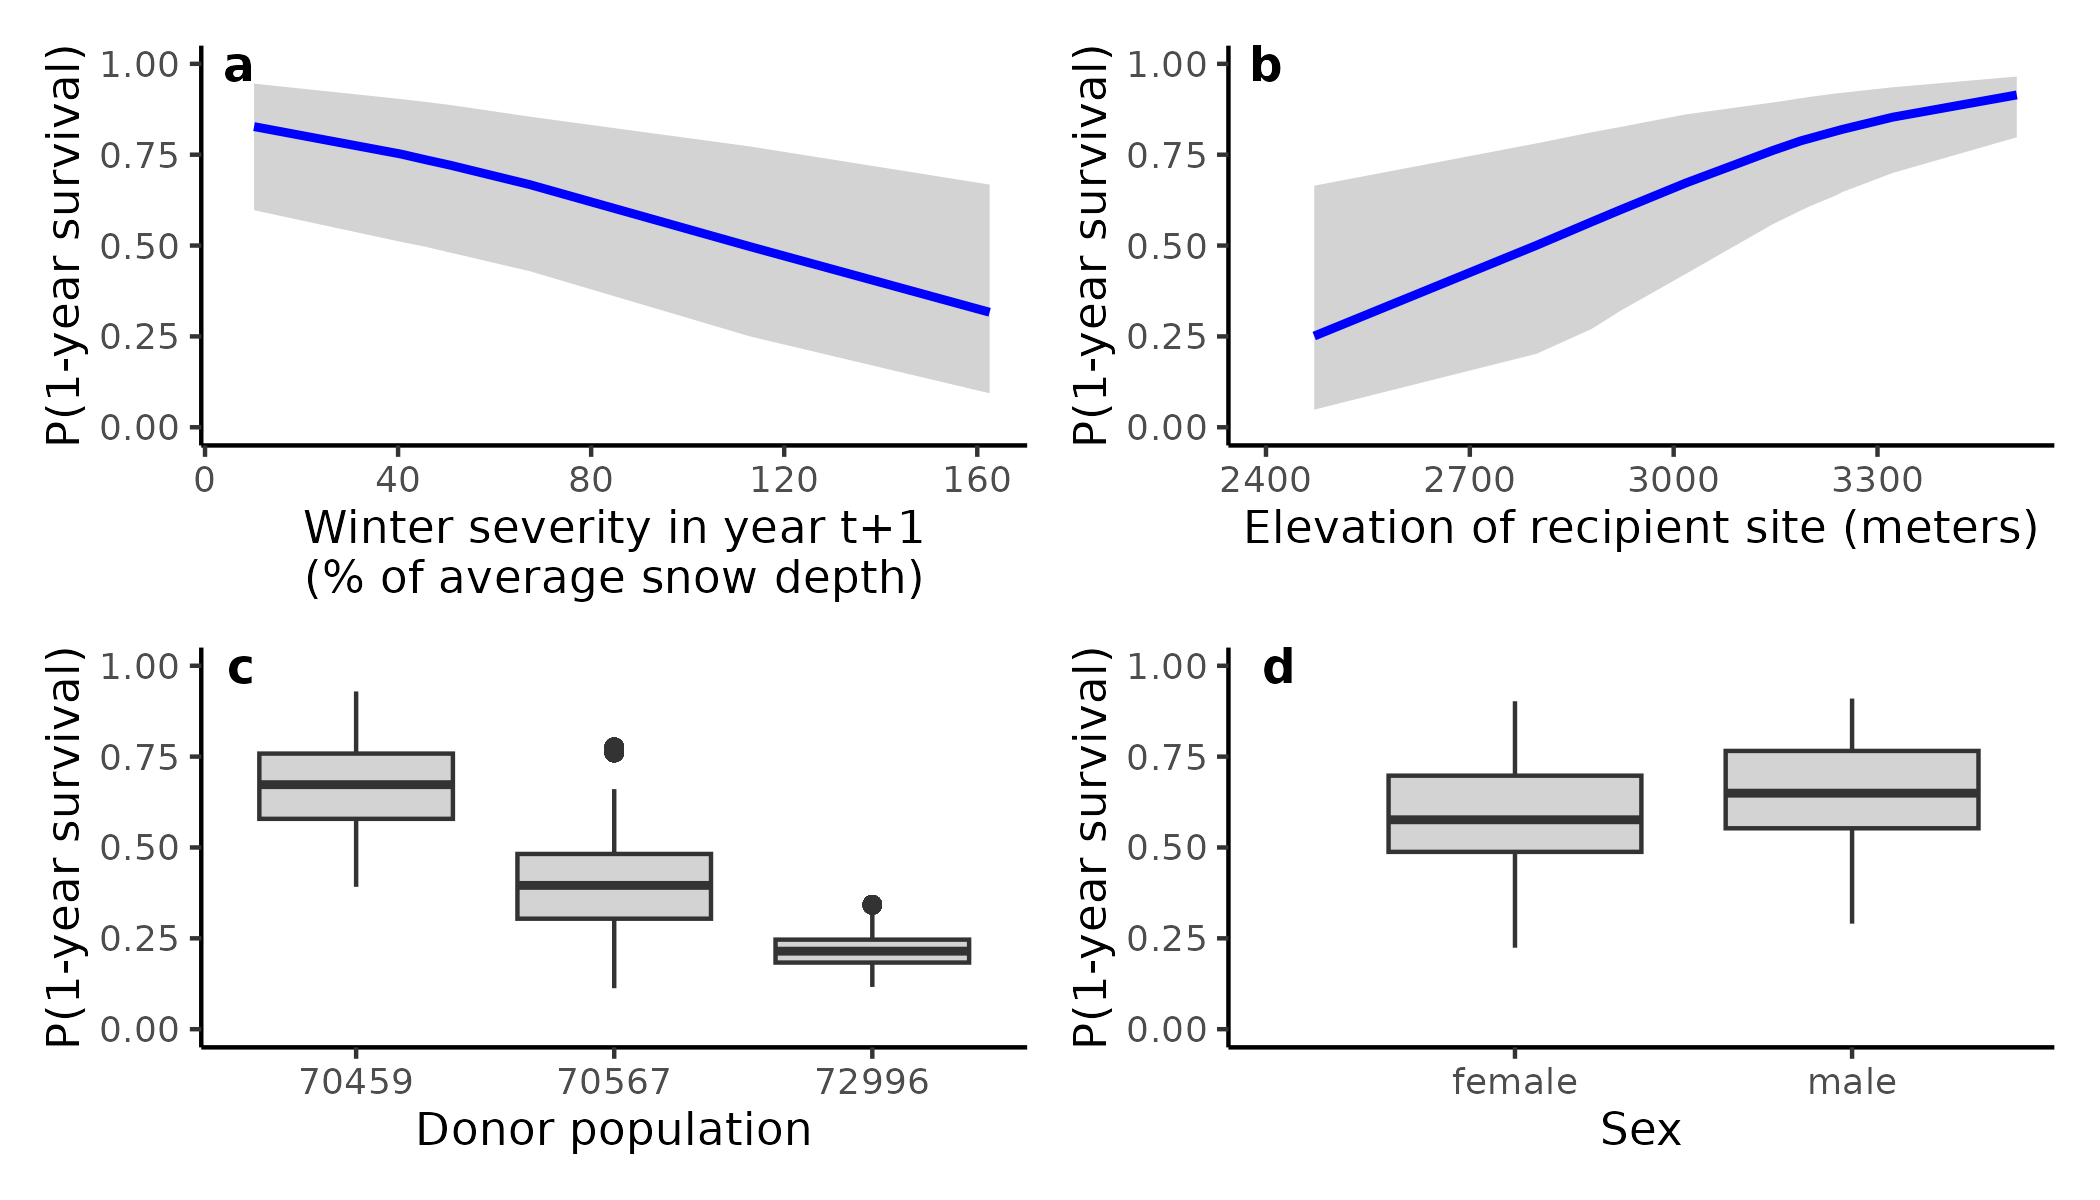
\includegraphics[width=\textwidth]{figures/cond_effects_plot.png}

}

\caption{\label{fig-cond-effects}Results from the among-site
meta-analysis showing conditional effects of the important predictors of
1-year frog survival (expressed as a probability): (A) winter severity
in the year following translocation, (B) elevation of recipient site,
(C) donor population, and (D) sex. In (A) and (B), blue lines are
medians and gray ribbons are 95\% uncertainty intervals. In (C) and (D),
box plots show medians, first and third quartiles, largest and smallest
values within 1.5x interquartile range, and values outside the 1.5x
interquartile range.}

\end{figure*}

\newpage

\begin{figure*}

{\centering 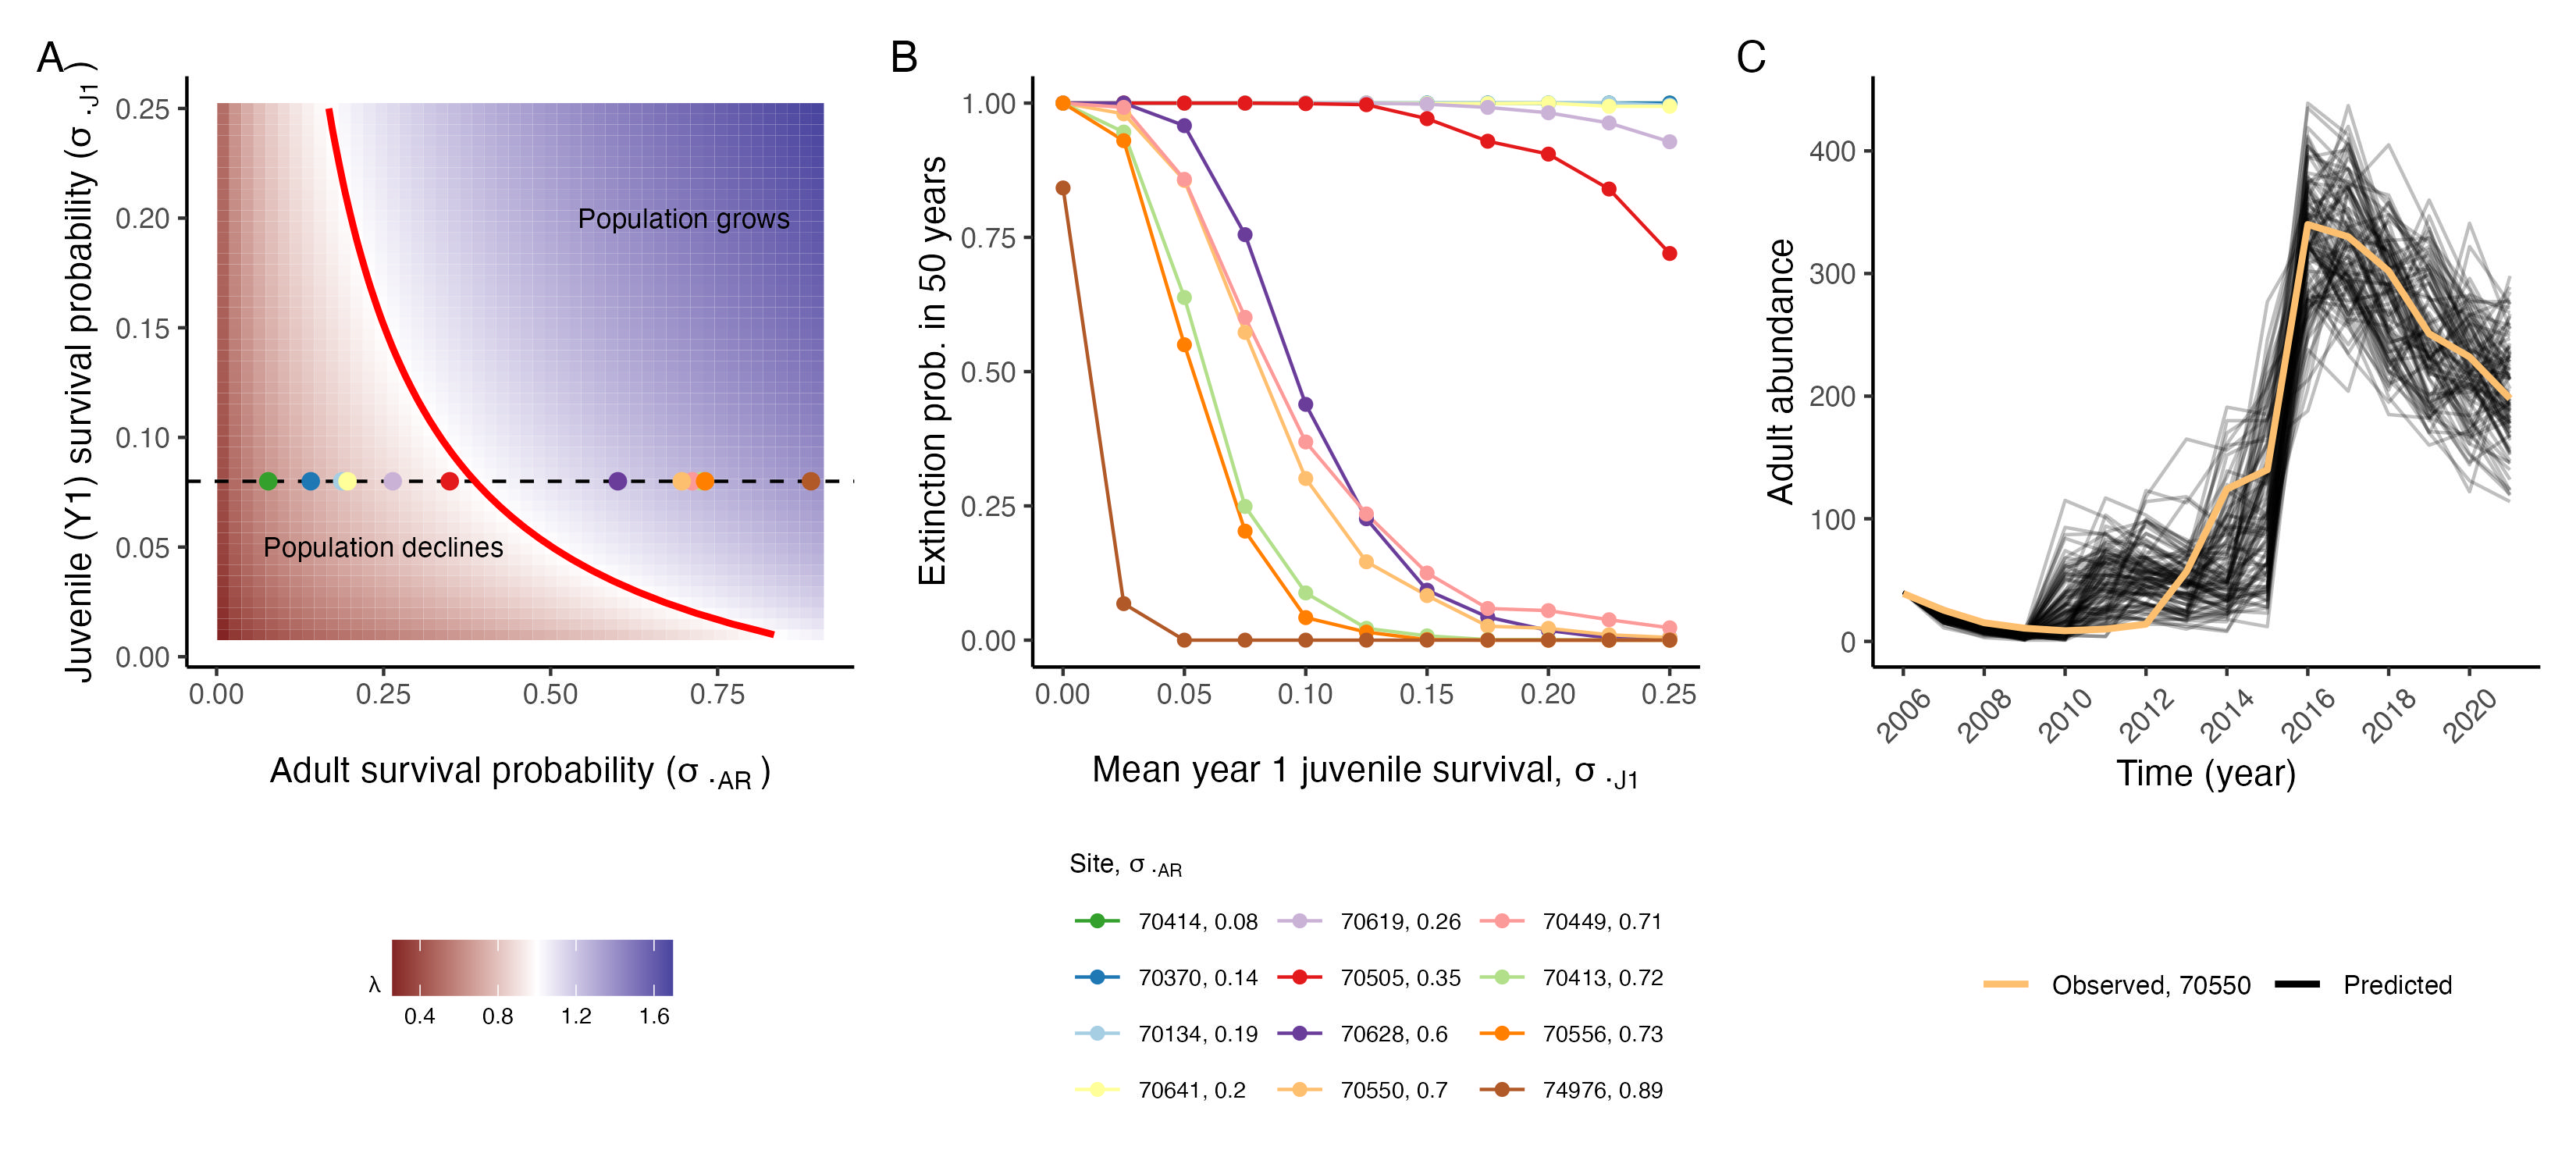
\includegraphics[width=\textwidth]{figures/pop_viability_figures_for_manuscript.jpg}

}

\caption{\label{fig-viability}Results from population viability
analysis: (A) Predicted long-run growth rate \(\lambda\) for different
values of yearly adult survival probability \(\sigma_{A_R}\) and year 1
juvenile survival and recruitment probability \(\sigma_{J_1}\), given
the parameterized, deterministic model. Colored points show the
predicted \(\lambda\) values for the twelve translocated populations
when year 1 juvenile survival probability is \(\sigma_{J_1} = 0.09\)
(indicated by the dashed line). The red line shows where
\(\lambda = 1\). Note that the point for 70413 is mostly hidden behind
other points. (B) Predicted 50-year extinction probabilities of the 12
translocated populations, given demographic stochasticity, environmental
variability in \(\sigma_{J_1}\), and different mean values of
\(\sigma_{J_1}\). There are 6 lines at extinction probability = 1, 5 of
which (70414--70619) are hidden beneath the line for 70505 when
\(\sigma_{J_1} < 0.10\). (C) 100 simulated trajectories (black lines)
from the population viability model that most closely matched the
observed abundance trajectory of adult amphibians at site 70550 (light
orange).}

\end{figure*}

\newpage

\begin{figure*}

{\centering 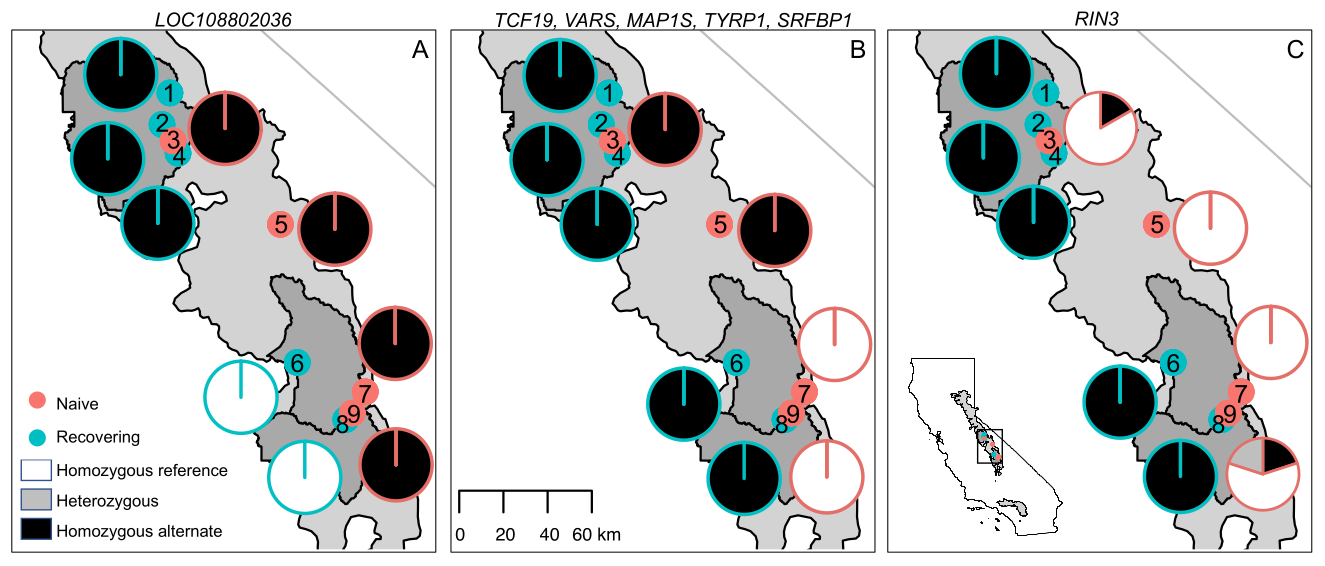
\includegraphics[width=\textwidth]{figures/allele_maps.png}

}

\caption{\label{fig-allelefrequencies}Evidence for selection on
individual variants in recovering MYL frog populations at the landscape
scale. For each of the 9 naive and recovering MYL frog populations
(indicated by numbered points), adjacent pie charts show allele
frequencies for the 11 outlier SNPs from 7 distinct genes: (A)
LOC108802036, (B) TCF19, VARS, MAP1S, TYRP1, and SRFBP1, and (C) RIN3.
Charts are superimposed on a map of the Sierra Nevada study area, with
Yosemite, Kings Canyon, and Sequoia National Parks (from north to south)
shown in dark gray, and the range boundary for MYL frogs shown in light
gray. The inset map locates the study area and range boundary in
California. Sites 1 and 4 (site id = 72996 and 70567, respectively) were
also used as sources of frogs in the frog population recovery study.}

\end{figure*}

\newpage

\begin{figure*}

{\centering 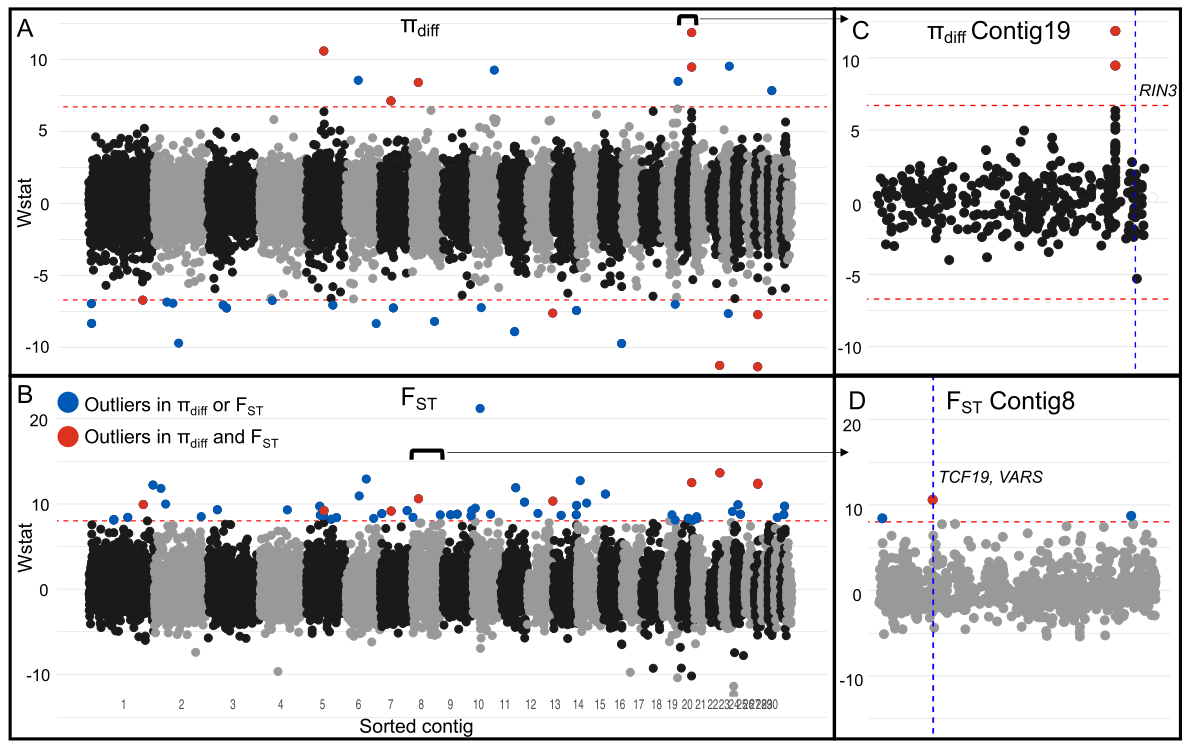
\includegraphics[width=\textwidth]{figures/splinewindow_manhattan.png}

}

\caption{\label{fig-spline-manhattan}Evidence for selection on genomic
regions in recovering MYL frog populations. Manhattan plot of the
results from the splined window analysis showing outlier regions for the
difference in (A) nucleotide diversity \(\pi_{diff}\) and (B)
\emph{F\textsubscript{ST}}. In (A), outlier regions are shown above the
upper red dashed line and below the lower red dashed line. In (B),
outlier regions are shown above the single dashed red line. Outlier
regions for either \(\pi_{diff}\) or \emph{F\textsubscript{ST}} are
shown in blue and outlier regions for both \(\pi_{diff}\) and
\emph{F\textsubscript{ST}} are shown in red. (C) Magnified Contig19 from
(A) showing two adjacent outlier regions for \(\pi_{diff}\) 12.9Mb
upstream of the RIN3 outlier SNP (indicated with a dashed vertical blue
line). (D) Magnified Contig8 from from (B) showing the
\emph{F\textsubscript{ST}} outlier region that includes the outlier SNPs
TCF19 and VARS. This region of the genome contains 8 annotated genes
known to occur in the extended MHC Class I and III regions.}

\end{figure*}

\newpage
\end{document}

